\chapter{Development of recommendation system}
\section*{Introduction}
This chapter presents the architectural design, implementation method-
ology, and empirical evaluation of the hybrid recommendation system
developed for the VitamiNurse mobile application. The system employs
a multi-modal architecture that integrates collaborative filtering, content-based filtering, and real-time behavioral analytics to deliver personalized
nutritional recommendations aligned with users’ health profiles, dietary
restrictions, and preferences.
The chapter begins with an analysis of vector databases as foundational
infrastructure for semantic retrieval, including a detailed discussion of approximate nearest neighbor (ANN) search and the Hierarchical Navigable
Small World (HNSW) algorithm. Subsequent sections detail the system’s
hybrid architecture, algorithmic components, embedding strategies, and
deployment pipeline.


\section{Vector Databases and Semantic Retrieval}
Vector databases serve as the backbone of modern content-based recommendation systems by enabling efficient similarity search in high-dimensional embedding spaces. In VitamiNurse, they facilitate the semantic matching of user health profiles with nutritional products based on dietary needs, allergies, and wellness goals.

\subsection{Fundamentals of Vector Databases}
Vector databases store and index dense numerical representations (embeddings) of data objects, allowing retrieval based on semantic similarity rather than exact keyword matches. 
Unlike relational databases, which organize data in tables, these systems represent data as vectors in a multi-dimensional space. 

\par These vectors encapsulate essential attributes of the items they represent, 
making vector databases ideal for tasks requiring similarity searches, nearest neighbor queries, and assessing distances or similarities between vectors \cite{IBMVectordb2025}. 
This capability is crucial in various applications, including recommendation systems, content-based image and video retrieval, and natural language understanding.

\begin{center}
\begin{figure}[H]
    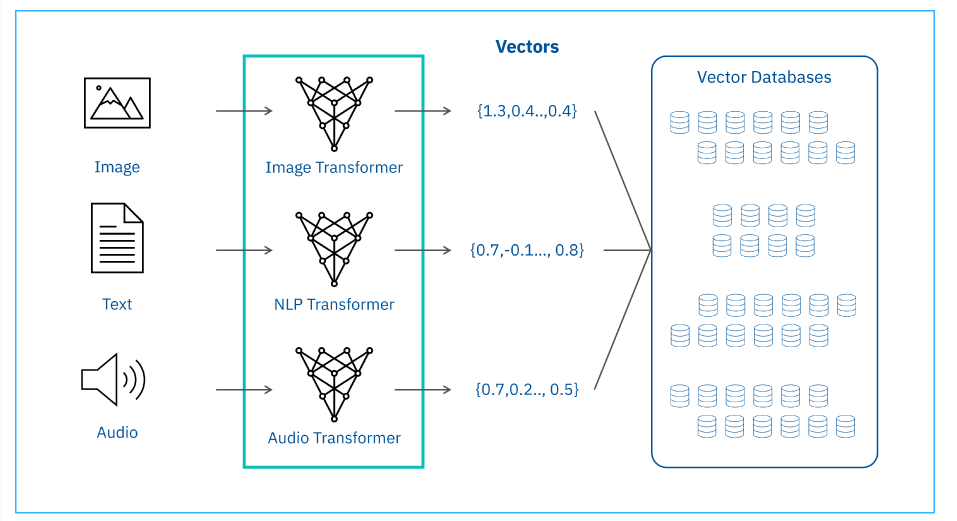
\includegraphics[scale=0.42]{images/vectorDB.png}
    \caption{Embedding representation in a vector database} 
    \label{fig:vectorDB_space}
\end{figure}
\end{center}

\subsection{Approximate Nearest Neighbor Search}
\par Based on comparing a query vector against all stored vectors, exact
similarity search becomes computationally prohibitive as dataset size
grows particularly in high-dimensional spaces due to the “curse of dimen-
sionality”\cite{ANN}. 
\par Approximate Nearest Neighbor (ANN) algorithms address this limitation
by sacrificing marginal accuracy for substantial gains in speed and memory
efficiency. These methods construct specialized index structures (e.g.,
trees, hash tables, or graphs) that enable sublinear-time retrieval of
near-optimal neighbors.

\subsection{The HNSW Algorithm}
Among ANN techniques, the Hierarchical Navigable Small World (HNSW)
algorithm has emerged as a state-of-the-art solution for large-scale similarity search\cite{HNSW}. HNSW organizes vectors into a multi-layer graph: upper
layers contain sparse, long-range connections for rapid coarse navigation,
while lower layers provide dense, local links for fine-grained refinement.
Search begins at the top layer and descends iteratively, achieving logarithmic time complexity with high recall. This balance of speed and
accuracy makes HNSW ideal for real-time recommendation systems.

\subsection{Selection of ChromaDB}
ChromaDB was selected as the vector database for VitamiNurse due to
its native support for HNSW indexing and native support for HNSW
indexing under an open-source license\cite{chromadocs2025}. A critical feature is its ability
to update the vector index dynamically without full retraining, which is
essential for the system’s daily synchronization of product metadata from
external retailers. Additionally, ChromaDB supports metadata filtering
alongside vector search, allowing post-retrieval enforcement of health
constraints such as excluding gluten-containing products for celiac users.

\begin{center}
\begin{figure}[H]
\centering
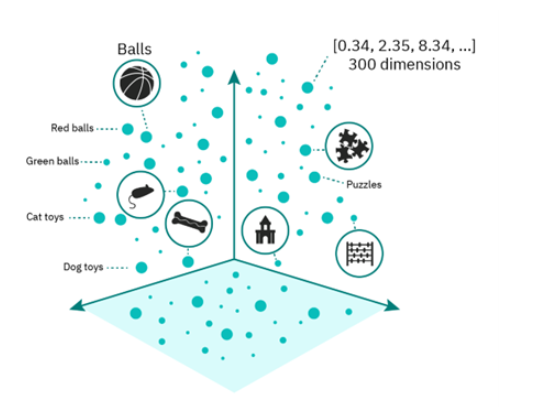
\includegraphics[scale=0.65]{images/chroma_space.png}
\caption{Vector search mechanism in ChromaDB} 
\label{fig:vectorDB}
\end{figure}
\end{center}

\subsection{Vector Search Versus Traditional Keyword Search}

Traditional search relies on discrete tokens and exact matching, limiting
its ability to generalize across semantically related terms. In contrast,
vector search retrieves items based on embedding proximity. For example,
a query for “dark chocolate” may return “organic cacao snacks” if their
embeddings are close, even in the absence of shared keywords. This
capability is essential for delivering nutritionally appropriate alternatives
that align with user health objectives.

\subsection{Embedding Generation}
Dense vector representations are produced using transformer-based sentence encoders. These models map textual descriptions of products and
user profiles into fixed-dimensional spaces where semantic relationships
are preserved geometrically. Efficient indexing and retrieval of these
embeddings are enabled by ANN algorithms such as HNSW, ensuring
scalability without compromising relevance.


\section{System Architecture}
VitamiNurse employs a \textbf{modular hybrid architecture}, separating collaborative and content-based filtering into specialized components:
\begin{itemize}
    \item \textbf{LightFM (Pure Collaborative)}: Captures long-term user preferences via matrix factorization, trained only on interaction data to avoid metadata-induced noise.
    \item \textbf{ChromaDB (Content-Based)}: Handles real-time product similarity using HNSW, enabling rapid updates without model retraining.
\end{itemize}

\subsection{Hybrid Architecture Design}

VitamiNurse implements a hybrid recommendation system that combines
offline collaborative filtering (CF) with real-time content-based filtering (CBF). The collaborative component uses LightFM, trained
nightly at 00:00 on user interaction data (views, likes, dislikes) to capture
long-term preferences without metadata bias. In parallel, a content-based pathway leverages ChromaDB with HNSW indexing to perform
low-latency similarity searches over product embeddings generated by
the all-MiniLM-L6-v2 model.

\begin{center}
\begin{figure}[H]
    \includegraphics[scale=0.35]{images/VN_recommendation.png}
    \caption{Recommendation System Architecture } 
    \label{fig:Recommendation_Sequence_Diagram}
\end{figure}
\end{center}

\par When a user scans a product, the system retrieves semantically similar items and re-ranks them according to the nutrition profile of the user.
This profile is continuously updated in real-time by its interactions with
the Nutrition AI Assistant.
Final recommendations are produced via a weighted ensemble (60\% content-based, 40\% collaborative), prioritizing immediate nutritional
relevance while retaining historical preference signals. The architecture is
organized into four layers—data ingestion, embedding generation, hybrid
recommendation, and API serving—enabling scalable, responsive, and health-conscious personalization.


\subsection{Hybrid System with Decoupled Components}

Although the LightFM framework supports two principal modes : \textbf{pure collaborative filtering} and \textbf{hybrid filtering}, we chose to employ only the pure collaborative model for VitamiNurse’s recommendation system.

This decision was made after extensive evaluation and careful alignment with the platform’s real-time infrastructure requirements. The selected approach offers greater scalability and modularity, particularly given the dynamic nature of our product catalog and metadata. 
The following subsections outline the key architectural and empirical factors that guided this choice.


\subsubsection{Why Not LightFM Hybrid?}

While hybrid models are often assumed to enhance performance by incorporating additional features, we avoided LightFM's hybrid mode for the following reasons:

\paragraph{1) Real-time Product Updates and Scalability Requirements :}
VitamiNurse's product database synchronizes daily with external retail inventories, meaning metadata (e.g., categories, availability) can change frequently. A hybrid LightFM model would require retraining whenever item features update, introducing latency and scalability challenges. In contrast, our content-based filtering module (powered by ChromaDB with HNSW-based approximate nearest neighbor search) dynamically adapts to metadata changes without retraining, making it better suited for real-time updates \cite{chromadb}.

ChromaDB's vector infrastructure is optimized for large-scale similarity search, supporting millions of product embeddings with efficient retrieval. This eliminates the need to encode metadata directly into LightFM, as the content-based component handles this asynchronously and with lower computational overhead.

\paragraph{2) Benchmark Evidence: Pure LightFM Outperforms Hybrid LightFM:}
Empirical studies consistently demonstrate that LightFM's pure collaborative model achieves superior performance compared to its hybrid counterpart:
\begin{itemize}
    \item \textbf{MovieLens 100k Benchmark}: \cite{shu2023lightfm} evaluated LightFM on the MovieLens dataset, showing that the pure model outperformed the hybrid variant in precision@K and recall@K across cutoffs (K=5, 10, 20). The hybrid model not only underperformed but also failed to surpass simpler baselines like ItemKNN in some metrics as illustrated in Figure~\ref{fig:precision}.

    \item \textbf{Feature Noise}: The inclusion of item features degraded performance, likely due to redundant or poorly weighted metadata. \cite{shu2023lightfm} found that the hybrid model's precision@5 was worse than graph-based baselines like P3$\alpha$ and RP3$\beta$.
    \item \textbf{Community Reports}: GitHub issues and user reports corroborate these findings, with cases where shuffled or irrelevant item features further reduced model accuracy \cite{lightfmissues}.
\end{itemize}
\begin{figure}[h!]
    \centering
    \begin{minipage}{0.49\textwidth}
        \centering
        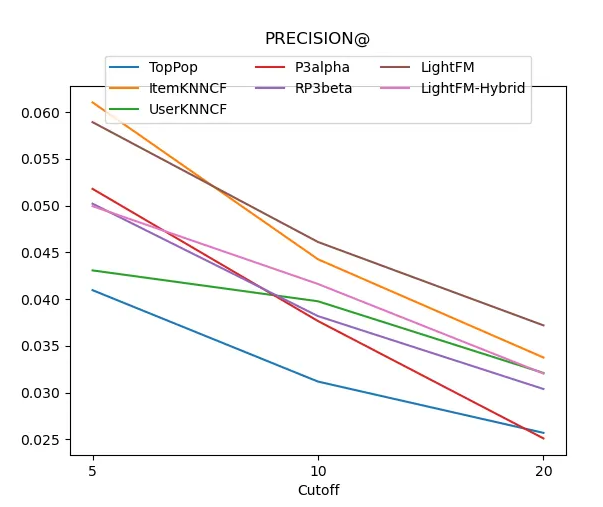
\includegraphics[width=\linewidth]{images/precision_plot.png}
        \caption{Cutoff Precision Values by Algorithm}
        \label{fig:precision}
    \end{minipage}\hfill
    \begin{minipage}{0.49\textwidth}
        \centering
        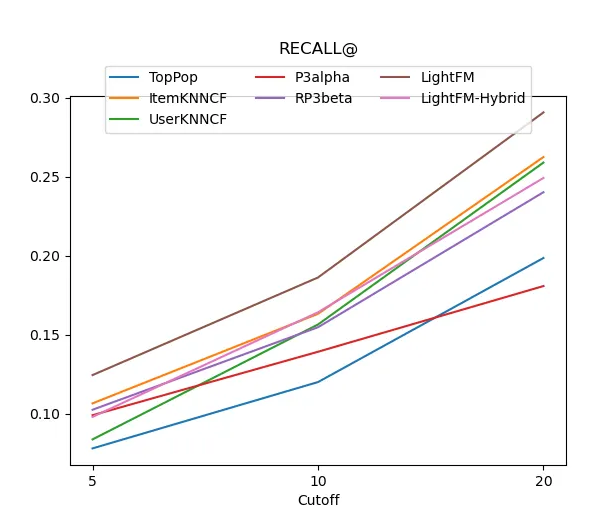
\includegraphics[width=\linewidth]{images/recall_plot.png}
        \caption{Cutoff Recall Values by Algorithm}
        \label{fig:recall}
    \end{minipage}
\end{figure}


\paragraph{3) Computational Efficiency :}
Pure collaborative filtering requires fewer computational resources during training and inference. Benchmarks on the Movielens 20M dataset show that LightFM's inference speed scales linearly with latent factor dimensionality, but hybrid models introduce additional overhead from feature processing.


This decoupling aligns with industry best practices, where hybrid \textit{systems} (not hybrid \textit{models}) often deliver more robust performance. This architecture ensures scalability while maintaining interpretability and efficiency.

\subsection{Dynamic Data Update and Sync Architecture}

The VitamiNurse system operates through a robust, modular data pipeline designed for real-time responsiveness and adaptability to both user behavior and product catalog changes:

\begin{enumerate}
    \item \textbf{Real-time Interaction Tracking}: User activities, such as viewing, liking, and disliking products, are continuously monitored and recorded. These interactions directly inform the recommendation engine, ensuring up-to-date and personalized  suggestions.
    
    \item \textbf{Dynamic Profile Synchronization}: Upon any profile change (e.g., allergy updates, changed health conditions, pregnancy status), the system triggers immediate re-embedding of the user's profile vector within ChromaDB. This ensures atomic, consistent updates that instantly reflect in recommendations, without disrupting the user's session.
    
    \item \textbf{Automated Product Ingestion and Embedding}: The product catalog is synchronized daily with partner retailers. New or modified products are automatically detected, vectorized through semantic embedding, and integrated into the recommendation graph using a CDC (Change Data Capture) pipeline.
    
    \item \textbf{Daily Model Retraining}: To adapt to evolving user preferences and product changes, the LightFM recommendation model is retrained every 24 hours (scheduled at 00:00 UTC). This ensures continuous learning and optimal recommendation quality.
\end{enumerate}

\vspace{1cm}

\section{content-based filtering}
The content-based (CB) recommendation module in \textit{VitamiNurse} is designed to provide personalized nutritional product suggestions by leveraging semantic similarity between user profiles and product characteristics. This is achieved through dense vector embeddings stored in ChromaDB and computed using a lightweight sentence-transformer model.
\begin{figure}[H]
    \centering
    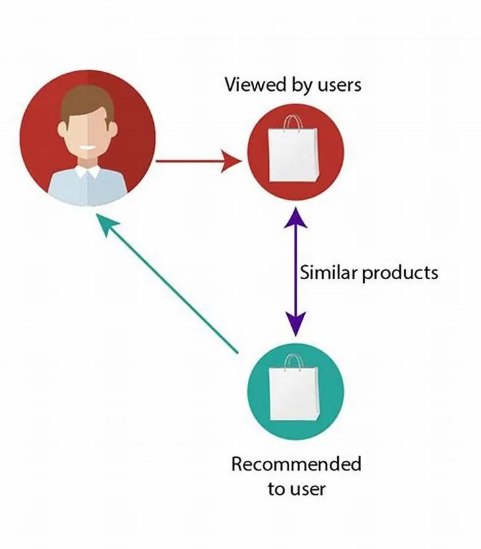
\includegraphics[scale=0.45]{images/cb_filtering_logic.png}
    \caption{Content Based Filtering Logic} 
    \label{fig:CB_filtering_logic}
\end{figure}


\subsection{Embedding Model Evaluation}

The \textit{SentenceTransformers} library offers a range of models evaluated for their performance in generating sentence embeddings and conducting semantic search, based on two key criteria: the quality of cross-sentence representations across 14 datasets and the effectiveness in semantic search tasks on 6 datasets.

 The \textbf{all-*} models, trained on an extensive corpus of over one billion text pairs, are designed as general-purpose models, with \texttt{all-mpnet-base-v2} delivering the highest overall quality and \texttt{all-MiniLM-L6-v2} providing comparable quality at approximately five times the speed, making it an efficient choice for various applications \cite{sbert2025models}.

\begin{table}[h!]
\centering
\resizebox{0.9\textwidth}{!}{%
\begin{tabular}{@{}lccccc@{}}
\toprule
\textbf{Model Name} & \textbf{Sent. Emb.} & \textbf{Sem. Search} & \textbf{Avg. Perf.} & \textbf{Speed} & \textbf{Size} \\
\midrule
\textbf{all-mpnet-base-v2} & \textbf{69.57} & \textbf{57.02} & \textbf{63.30} & \textbf{2800} & 420 MB \\
multi-qa-mpnet-base-dot-v1 & 66.76 & 57.60 & 62.18 & 2800 & 420 MB \\
all-distilroberta-v1 & 68.73 & 50.94 & 59.84 & 4000 & 290 MB \\
all-MiniLM-L12-v2 & 68.70 & 50.82 & 59.76 & 7500 & 120 MB \\
multi-qa-distilbert-cos-v1 & 65.98 & 52.83 & 59.41 & 4000 & 250 MB \\
\textbf{all-MiniLM-L6-v2} & \textbf{68.06} & \textbf{49.54} & \textbf{58.80} & \textbf{14200} & 80 MB \\
multi-qa-MiniLM-L6-cos-v1 & 64.33 & 51.83 & 58.08 & 14200 & 80 MB \\
paraphrase-multilingual-mpnet-base-v2 & 65.83 & 41.68 & 53.75 & 2500 & 970 MB \\
paraphrase-albert-small-v2 & 64.46 & 40.04 & 52.25 & 5000 & 43 MB \\
paraphrase-multilingual-MiniLM-L12-v2 & 64.25 & 39.19 & 51.72 & 7500 & 420 MB \\
paraphrase-MiniLM-L3-v2 & 62.29 & 39.19 & 50.74 & 19000 & 61 MB \\
distiluse-base-multilingual-cased-v1 & 61.30 & 29.87 & 45.59 & 4000 & 480 MB \\
distiluse-base-multilingual-cased-v2 & 60.18 & 27.35 & 43.77 & 4000 & 480 MB \\
\bottomrule
\end{tabular}
}
\caption{Performance comparison of SentenceTransformer models. Speed is measured as average sentences processed per second.}
\label{tab:models}
\end{table}

 
\subsection{Embedding Model Selection}
\par The system employs the all-MiniLM-L6-v2 model for generating embeddings, which offers several advantages over alternatives. 
By being fine-tuned on over 1 billion text pairs, the all-MiniLM-L6-v2 excels in semantic similarity tasks. 
Despite its smaller size,it achieves 93\% the accuracy of larger models such as BERT-base models. 

\par This sentence transformer model is an excellent choice for VitamiNurse recommendation system, as it produces 384-dimensional embeddings that effectively capture subtle relationships within the data \cite{allMiniLML12}. Furthermore, its compact architecture, with only 33.4 million parameters, enables
efficient CPU-only inference, and multilingual support enables global applicability, making it
perfect for delivering fast and accurate recommendations.


\subsection{CB Recommendation Process}
 The content-based recommendation process in VitamiNurse involves several key steps to generate personalized product suggestions based on user profiles and scanned items.
\subsubsection{Query Construction}
\par The CB system operates based on two possible inputs: the \textbf{user identifier} and an optional \textbf{scanned product identifier} (EAN code). When a user scans a product, the system retrieves metadata associated with that item such as product name, brand, categories, and nutrition information. Simultaneously, it extracts the user’s profile information, which includes dietary preferences, pregnancy status, and medical conditions like diabetes or hypertension.\\
These two sources of information are merged to create a descriptive query that captures both the scanned product’s features and the user's health-related needs. 

\subsubsection{Search and Recommendation}
The query is then embedded into a vector using the selected embedding model and used to perform a semantic search in the product database. The search returns a list of nutritionally and semantically similar products.
\par In cases where no product is scanned, the recommendation relies entirely on the user’s profile to infer their preferences and health requirements. Based on this information, it generates a personalized query, which is then used to display tailored recommendations on the home page.


\subsubsection{Recommendation Score}
\par Each recommended product is assigned a relevance score based on semantic proximity. This score is further refined by applying domain specific nutritional rules by boosting products with better Nutri-Scores. The system also applies post-filtering to strictly enforce compatibility with medical conditions or dietary restrictions. For instance, a user with celiac disease will never be recommended a product that contains gluten, even if it is semantically similar.

\subsubsection{CB Recommendation Workflow :}
The content based recommendation workflow follows a structured process in order to offer a personalized and health-aware user experience, as illustrated in the following diagram. It begins by metadata gathering and query construction. Queries are embedded into vectors using the all-MiniLM-L6-v2 model for semantic search against the product database. The system then selects and returns recommendations aligned with user preferences and nutritional needs.


\par This design ensures that the products delivered by the content based recommendation system are not only contextually relevant but also aligned with the unique nutritional profile of each user of \textit{VitamiNurse} app.

\vspace{0.4cm}
\section{Collaborative Filtering}
Collaborative filtering in \textit{VitamiNurse} leverages the \textbf{LightFM} model, which combines matrix factorization and metadata-aware learning. 
\subsection{Overview}

Collaborative filtering (CF) is a widely used recommender system technique that predicts user preferences by leveraging the collective behavior of similar users or items. As defined by IBM, CF operates on the principle that users with shared interests in the past will likely agree in the future, making recommendations based on patterns identified in user-item interaction matrices\cite{ibmCF}.

\begin{center}
    \begin{figure}[H]
        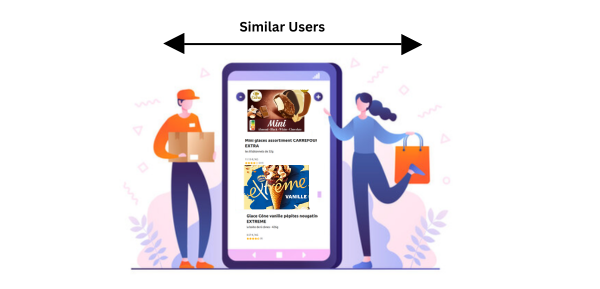
\includegraphics[scale=0.95]{images/collaborative_filtering.png}
        \caption{Collaborative Filtering Logic}
        \label{fig:cf_workflow}
    \end{figure}
\end{center}

\subsection{LightFM's Collaborative Filtering Approach}
LightFM  implements a hybrid matrix factorization model rather than traditional memory-based (neighborhood) collaborative filtering. Unlike user/item-neighborhood methods that rely on cosine similarity or Pearson correlation \cite{ibmCF}, LightFM learns latent embeddings using Weighted Matrix Factorization (WMF) or Bayesian Personalized Ranking (BPR) loss. This approach is scalable and well-suited for sparse datasets, making it ideal for recommendation systems like VitamiNurse.

\subsection{Create the interaction matrix}
VitamiNurse incorporates multiple types of user feedback, each assigned specific weights to reflect varying degrees of preference:

\begin{table}[h]
\centering
\begin{tabular}{lcc}
\toprule
\textbf{Interaction Type} & \textbf{Weight} & \textbf{Interpretation} \\
\midrule
Liked & 1.0 & Strong positive preference \\
Visited & 0.5 & Mild interest/engagement \\
Disliked & -1.0 & Explicit negative feedback \\
\bottomrule
\end{tabular}
\caption{User Interaction Types and Their Weighting in VitamiNurse}
\label{tab:interaction_weights}
\end{table}

\subsection{Loss Functions in LightFM}

The LightFM library supports multiple loss functions tailored to different recommendation scenarios:
\begin{itemize}
    \item \textbf{WARP} (Weighted Approximate-Rank Pairwise): Optimized for ranking tasks with implicit feedback (clicks). It focuses on positive signals and is effective for top-N recommendations but does not handle negative feedback well.
    \item \textbf{BPR} (Bayesian Personalized Ranking): Designed for personalized item ranking through pairwise comparisons. It ranks preferred items higher than less preferred or irrelevant ones, accommodating nuanced feedback.
    \item \textbf{Logistic}: Used for probabilistic modeling, typically with explicit feedback (ratings)
\end{itemize}

\subsection{Selection of Loss Function}

\par The selection of an appropriate loss function is critical in recommendation
systems, as it determines how user-item interactions are modeled during
the training process. Collaborative filtering leverages implicit feedback
(likes, views, dislikes) weighted as shown in Table \ref{tab:interaction_weights} to inform this
process.
\par Our collaborative module cannot use WARP loss because it fails to model
explicit dislikes (-1.0). Instead, Bayesian Personalized Ranking
(BPR) was chosen because it optimizes pairwise comparisons, explicitly
ranking liked items higher than visited or disliked ones while leveraging
both positive and negative signals. This approach better aligns with
VitamiNurse’s goal of learning from complex user interactions while
maintaining scalability on sparse datasets.

\vspace{0.5cm}
\section{Benchmarking the Recommendation System: Exact vs. ANN (HNSW) Search}

To ensure both scalability and precision, we benchmarked two vector search modes available in ChromaDB: the default exact search and the HNSW-enabled Approximate Nearest Neighbor (ANN) search.

\subsection{Theoretical Comparison}
\par Exact search is ChromaDB’s default method . It performs exhaustive comparisons between the query vector and all stored vectors using cosine similarity, ensuring maximum precision. However, this method can become computationally expensive as the dataset grows.

\par As we have seen, HNSW search is an approximate nearest neighbor (ANN) technique that is frequently adopted in large-scale recommender systems. It constructs a navigable graph index that accelerates retrieval. Although it introduces a slight drop in precision, it significantly enhances speed and scalability.

\noindent
The following table summarizes the key differences between the two modes:

\begin{table}[h!]
\centering
\resizebox{0.9\textwidth}{!}{%
\begin{tabular}{|l|c|c|}
\hline
\textbf{Feature} & \textbf{Default (Exact Search)} & \textbf{HNSW (ANN)} \\
\hline
Accuracy & 100\% precise & Approximate (configurable) \\
\hline
Speed & Slow for large datasets & Faster, scales better \\
\hline
Memory & Lower overhead & Higher (stores graph index) \\
\hline
Use Case & Small datasets ($<$10K vectors) & Large datasets \\
\hline
\end{tabular}
}
\caption{Key Differences: Default vs. HNSW Search}
\label{tab:theoretical-comparison}
\end{table}

\subsection{Experimental Results and Scalability Implications}

We benchmarked 20,000 recommendation requests using ChromaDB with 23,000 products indexed. Both modes—Exact (port \texttt{8000}) and HNSW (port \texttt{8001})—returned valid top-10 results for each request with a 100\% success rate.

\begin{table}[H]
\centering
\caption{Benchmark Results for Recommendation Modes}
\label{tab:benchmark-results}
\resizebox{0.9\textwidth}{!}{%
\begin{tabular}{|l|c|c|c|}
\hline
\textbf{Mode} & \textbf{Avg Time (ms)} & \textbf{Avg Results} & \textbf{Success Rate (\%)} \\
\hline
Exact (8000) & 187.4 & 10 & 100.0 \\
HNSW  (8001) & 178.08 & 10 & 100.0 \\
\hline
\end{tabular}
}
\end{table}

\par Results demonstrate that \textbf{HNSW} significantly outperforms exact search in terms of speed (from 1$87.4$ms to $178.08$ms), even with only 23,000 products. As VitamiNurse scales to hundreds of thousands or even millions of products across Europe and the US, the cost of exact search will become increasingly prohibitive.

\par HNSW, by contrast, offers scalable performance with near-equivalent accuracy, making it the preferred choice for large-scale deployments in real-time production environments.


\par Results demonstrate that \textbf{HNSW} significantly outperforms \textbf{exact search} on speed while maintaining high relevance in practical use cases. It is now the preferred mode for large-scale deployments in VitamiNurse.

\vspace{1cm}
\section{Deployment}
The recommendation system is deployed as a RESTful API using FastAPI, enabling seamless integration with the VitamiNurse mobile application. This section outlines the deployment architecture and multi-modal recommendation capabilities.

\subsection{FastAPI Deployment}
To facilitate real-time access to personalized nutritional recommendations within the \textit{VitamiNurse} mobile application, the recommendation engine is exposed through a RESTful API developed using a private \textbf{FastAPI} service. We chose FastAPI for its performance, asynchronous capabilities, and automatic data validation using Pydantic.\\

\par Our API provides a single endpoint, /recommend, which receives structured input from the application (user ID, scanned EAN,limit, recommendation\_type) and returns tailored food item suggestions in JSON format.


\subsection{Multi-Modal recommendation deployment}
The API supports three recommendation modes selectable via a \texttt{recommendation\_type} parameter: 
\begin{enumerate}
    \item Collaborative filtering
    \item Content-based filtering
    \item Hybrid approach
\end{enumerate}

This internal service ensures fast, reliable, and scalable communication between the application and the recommendation system. Although fully documented through FastAPI’s auto-generated Swagger UI, the API will be accessed exclusively by the mobile application and the development team for testing.
 \begin{center}
    \begin{figure}[H]
        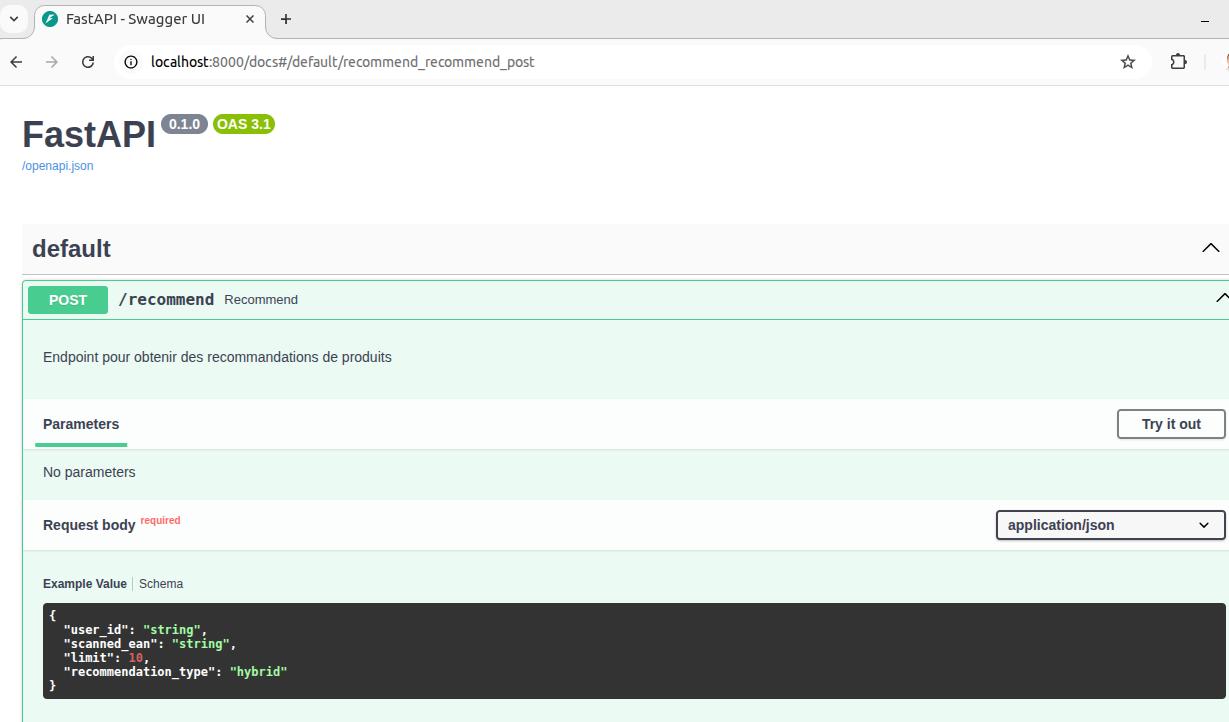
\includegraphics[scale=0.41]{images/swaggerFastAPI.png}
    \caption{Swagger UI for the internal Recommendation API} 
    \label{fig:swagger_UI}
\end{figure}
\end{center}

\section*{Conclusion}
This chapter has outlined the architectural and algorithmic foundations of the VitamiNurse recommendation system. 
The system employs a modular, hybrid architecture that separates collaborative and content-based filtering to achieve a balance between scalability and precision. 
Integration of ChromaDB with HNSW indexing facilitates efficient semantic analysis of user needs and product attributes. 
Additionally, the LightFM model, trained using a Bayesian Personalized Ranking (BPR) loss function, effectively captures dynamic user preferences derived from implicit feedback.

By concentrating on the user health condition, allergies and health goals, the recommendation system suggests more healthy and personalized products. However, providing effective guidance also requires an intuitive and interactive tool. To address this need, the next chapter introduces VitamiNurse AI assistant, designed to deliver real-time, conversational support that bridges large language models with user-friendly interaction.  
